\section{Introduction}

\subsection{Overview}

The NUbots from the University of Newcastle, Australia have had a strong record of success in the RoboCup Four Legged League since first entering in 2002. The Nubots achieved 3rd place in 2002 (Fukuoka), and again in 2003 (Padua) and 2004 (Lisbon). In 2005 (Osaka) with a complete redevelopment of the code, the NUbots came 2nd in a heartbreaking penalty shoot out against the German Team. With a strong 2005 base code, 2006 development focused on debugging and fine tuning. The result was a nail biting final against rUNSWift in Bremen where the NUbots won 7-3. Code development plateaued in 2007 and we lost the final in Atlanta against the Northern Bites, a relatively new team who was heavily influenced by our methods.  

2008 was a year of change. The transition from the Sony ERS-7 robot to the Aldebaran Nao meant a total rewrite of the software system. In addition, two of our main team members left. Michael Quinlan was `poached' by UT Austin and Rick Middleton moved to the National University of Ireland, Maynooth (NUIM). With a limited number of places available in the new Nao League we decided to collaborate with Rick and NUIM to form a joint team, the `NUManoids'. 

2008 was also a year of challenges. University payment issues, spliting the robot package and repair delays meant even that we had even less time to work on the robot than originally planned. In the end we had approximately 3 weeks `hands on' time with a robot. International collaboration proved quite difficult in the short amount of development time. 

The NUManoids preparation stategy was based on priorities. Our first priority was to chase the ball. This required the robot to see the ball, track the ball and walk towards the ball. 

Our next aim was to kick towards a goal. Unfortunately we didn't get a chance to implement this. Time restrictions and international collaboration meant that the integration of localisation was delayed until we arrived at the venue. We did not get a chance to properly test localisation hence we could not write behaviour that depended on it. However, by the final we had implemented behaviour that attempted to not kick towards our own goal. 

A heightened stance and reduced stiffness of the joints was our advantage in game performance. Our walk style also doubled as a kick. Our walk comprised of short sharp steps so there was no need to waste time lining up the ball for a kick. Our behaviour concept was to at least do something with the ball and get rid of it as quickly as possible. 


\subsection{Software Layout}

Our 2008 system was based on our Aibo architecture. Our system consists of one control module \emph{Nao} and four functional modules -
\emph{Vision, Localisation, Behaviour and
Locomotion}. 

The flow of information in our system can be seen in Figure
\ref{fig:software}. 

\begin{figure}[!h]
\begin{center}
    %\leavevmode
    \scalebox{0.5} {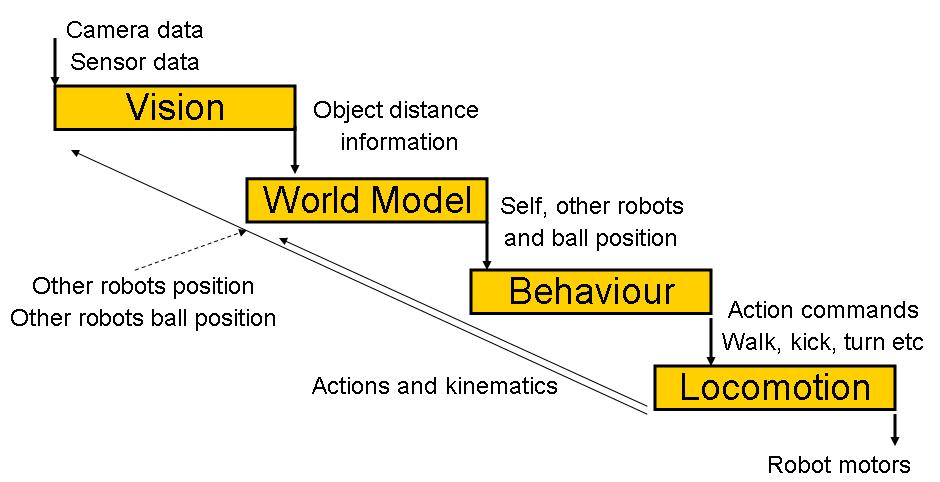
\includegraphics{figs/software.jpg} }
    \caption{2008 Software Architecture}
    \label{fig:software}
\end{center}
\end{figure}

